%====================================================%
% SEZIONE 1: Esercizi base sul MRUA
%====================================================%
\begin{question}[ID=1.1, subtitle={Automobile in accelerazione da fermo}, tags={mua, legge oraria}, difficulty=facile]
Un'automobile si trova inizialmente ferma. All'istante $t = 0$, il conducente accelera con $a = 2 \, \text{m/s}^2$ costante.
\begin{enumerate}
    \item Determina la velocità dell'automobile dopo $t = 5 \, \text{s}$.
    \item Calcola la distanza percorsa nei primi $5 \, \text{s}$.
\end{enumerate}
\begin{solution}
    \begin{enumerate}
        \item $v = v_0 + at = 0 + 2 \cdot 5 = 10 \, \text{m/s}$.
        \item $s = \tfrac{1}{2}at^2 = \tfrac{1}{2} \cdot 2 \cdot 25 = 25 \, \text{m}$.
    \end{enumerate}
\end{solution}
\end{question}

%------------------------------------------------------------------------------------%

\begin{question}[ID=1.2, subtitle={Treno merci in frenata uniforme}, tags={mua, frenata}, difficulty=facile]
Un treno merci viaggia a $v_0 = 10 \, \text{m/s}$ e frena con $a = -0{,}5 \, \text{m/s}^2$.
\begin{enumerate}
    \item Quanto tempo impiega il treno per fermarsi?
    \item Qual è la distanza percorsa durante la frenata?
\end{enumerate}
\begin{solution}
    \begin{enumerate}
        \item $0 = 10 - 0{,}5\,t \;\Rightarrow\; t = 20 \, \text{s}$.
        \item $s = v_0 t + \tfrac{1}{2}at^2 = 10 \cdot 20 - \tfrac{1}{2} \cdot 0{,}5 \cdot 400 = 200 - 100 = 100 \, \text{m}$.
    \end{enumerate}
\end{solution}
\end{question}

%------------------------------------------------------------------------------------%

\begin{question}[ID=1.3, subtitle={Ciclista che parte da fermo percorre 100 m}, tags={mua, accelerazione}, difficulty=facile]
Un ciclista parte da fermo e percorre $100 \, \text{m}$ in $10 \, \text{s}$ con accelerazione costante.
\begin{enumerate}
    \item Determina l'accelerazione mantenuta.
    \item Calcola la velocità al termine del tratto.
\end{enumerate}
\begin{solution}
    \begin{enumerate}
        \item $s = \tfrac{1}{2}at^2 \;\Rightarrow\; a = 2s/t^2 = 200/100 = 2 \, \text{m/s}^2$.
        \item $v = at = 2 \cdot 10 = 20 \, \text{m/s}$.
    \end{enumerate}
\end{solution}
\end{question}

%------------------------------------------------------------------------------------%

\begin{question}[ID=1.4, subtitle={Palla lanciata verticalmente verso l'alto}, tags={mua, caduta libera}, difficulty=facile]
Una palla è lanciata verticalmente con $v_0 = 20 \, \text{m/s}$; $a = -9{,}8 \, \text{m/s}^2$.
\begin{enumerate}
    \item Determina l'altezza massima raggiunta.
    \item Calcola il tempo per raggiungere l'altezza massima.
\end{enumerate}
\begin{solution}
    \begin{enumerate}
        \item $v^2 = v_0^2 + 2as \;\Rightarrow\; s = v_0^2/(2g) = 400/19{,}6 \approx 20{,}4 \, \text{m}$.
        \item $0 = 20 - 9{,}8t \;\Rightarrow\; t \approx 2{,}04 \, \text{s}$.
    \end{enumerate}
\end{solution}
\end{question}

%------------------------------------------------------------------------------------%

\begin{question}[ID=1.5, subtitle={Razzo in accelerazione costante per 20 s}, tags={mua, legge oraria}, difficulty=facile]
Un razzo parte da fermo e accelera con $a = 15 \, \text{m/s}^2$ per $t = 20 \, \text{s}$.
\begin{enumerate}
    \item Calcola la velocità finale.
    \item Calcola lo spazio percorso.
\end{enumerate}
\begin{solution}
    \begin{enumerate}
        \item $v = at = 15 \cdot 20 = 300 \, \text{m/s}$.
        \item $s = \tfrac{1}{2}at^2 = \tfrac{1}{2} \cdot 15 \cdot 400 = 3000 \, \text{m}$.
    \end{enumerate}
\end{solution}
\end{question}

%====================================================%
% SEZIONE 2: Quiz sul MRUA
%====================================================%
\begin{question}[ID=2.1, subtitle={Grandezza costante nel MRUA}, tags={mua}, difficulty=facile]
Quale grandezza rimane costante nel moto rettilineo uniformemente accelerato?

\vspace{0.5em}

\begin{tabularx}{\linewidth}{@{}X X X X@{}}
\boxed{A}\hspace{6pt} la velocità &
\boxed{B}\hspace{6pt} l'accelerazione &
\boxed{C}\hspace{6pt} lo spazio &
\boxed{D}\hspace{6pt} il tempo
\end{tabularx}
\begin{solution}
Risposta: \textbf{B}. Nel MRUA l'accelerazione è costante per definizione.
\end{solution}
\end{question}

\begin{question}[ID=2.2, subtitle={Unità di misura dell'accelerazione nel SI}, tags={mua}, difficulty=facile]
Qual è l'unità di misura dell'accelerazione nel Sistema Internazionale?

\vspace{0.5em}

\begin{tabularx}{\linewidth}{@{}X X X X@{}}
\boxed{A}\hspace{6pt} km/s &
\boxed{B}\hspace{6pt} km/h &
\boxed{C}\hspace{6pt} m/s &
\boxed{D}\hspace{6pt} m/s$^2$
\end{tabularx}
\begin{solution}
Risposta: \textbf{D}. L'unità SI dell'accelerazione è il metro al secondo quadrato ($\text{m/s}^2$).
\end{solution}
\end{question}

\begin{question}[ID=2.3, subtitle={Legge oraria del MRUA}, tags={mua}, difficulty=facile]
Quale tra queste è la legge oraria del moto rettilineo uniformemente accelerato?

\vspace{0.5em}

\begin{tabularx}{\linewidth}{@{}X X X X@{}}
\boxed{A}\hspace{6pt} $v = v_0 + at$ &
\boxed{B}\hspace{6pt} $s = s_0 + vt$ &
\boxed{C}\hspace{6pt} $s = s_0 + v_0t + \dfrac{1}{2}at^2$ &
\boxed{D}\hspace{6pt} $s = v_0t - \dfrac{1}{2}gt^2$
\end{tabularx}
\begin{solution}
Risposta: \textbf{C}. La legge oraria del MRUA è $s = s_0 + v_0t + \tfrac{1}{2}at^2$.
\end{solution}
\end{question}

\begin{question}[ID=2.4, subtitle={Grafico spazio-tempo del MRUA}, tags={mua}, difficulty=facile]
Nel grafico spazio-tempo di un moto rettilineo uniformemente accelerato, che funzione è rappresentata?

\vspace{0.5em}

\begin{tabularx}{\linewidth}{@{}X X X X@{}}
\boxed{A}\hspace{6pt} una retta &
\boxed{B}\hspace{6pt} una parabola &
\boxed{C}\hspace{6pt} una curva &
\boxed{D}\hspace{6pt} un punto
\end{tabularx}
\begin{solution}
Risposta: \textbf{B}. Poiché $s \propto t^2$, il grafico $s$-$t$ è una parabola.
\end{solution}
\end{question}

%====================================================%
% SEZIONE 3: Educazione Civica — spazio di arresto
%====================================================%
\begin{question}[ID=3.1, subtitle={Accelerazione durante una frenata}, tags={mua, frenata, spazio di arresto}, difficulty=media]
Durante una frenata l'accelerazione:

\vspace{0.5em}

\begin{tabularx}{\linewidth}{@{}X X@{}}
\boxed{A}\hspace{6pt} è nulla, altrimenti l'auto non potrebbe frenare \\
\boxed{B}\hspace{6pt} diminuisce gradualmente fino ad annullarsi \\
\boxed{C}\hspace{6pt} è limitata dalle condizioni del veicolo e della strada \\
\boxed{D}\hspace{6pt} aumenta gradualmente fino a un valore massimo
\end{tabularx}
\begin{solution}
Risposta: \textbf{C}. L'accelerazione di frenata dipende dall'attrito tra pneumatici e asfalto e dalle caratteristiche del sistema frenante; non è né nulla né crescente.
\end{solution}
\end{question}

\begin{question}[ID=3.2, subtitle={Proporzionalità della distanza di frenata}, tags={mua, frenata, spazio di arresto}, difficulty=media]
La distanza percorsa durante una frenata uniforme fino all'arresto:

\vspace{0.5em}

\begin{tabularx}{\linewidth}{@{}X X@{}}
\boxed{A}\hspace{6pt} è direttamente proporzionale alla velocità iniziale \\
\boxed{B}\hspace{6pt} è proporzionale al quadrato della velocità iniziale \\
\boxed{C}\hspace{6pt} è inversamente proporzionale alla velocità iniziale \\
\boxed{D}\hspace{6pt} dipende linearmente dalla velocità iniziale
\end{tabularx}
\begin{solution}
Risposta: \textbf{B}. Dalla formula $v^2 = v_0^2 + 2as$ con $v=0$: $s = v_0^2/(2|a|)$, proporzionale al quadrato della velocità iniziale.
\end{solution}
\end{question}

\begin{question}[ID=3.3, subtitle={Effetto del tempo di reazione sullo spazio di arresto}, tags={mua, frenata, spazio di arresto}, difficulty=media]
Il tempo di reazione:

\vspace{0.5em}

\begin{tabularx}{\linewidth}{@{}X X@{}}
\boxed{A}\hspace{6pt} non incide sullo spazio di arresto \\
\boxed{B}\hspace{6pt} incide in maniera trascurabile sullo spazio di arresto \\
\boxed{C}\hspace{6pt} incide in maniera significativa sullo spazio di arresto \\
\boxed{D}\hspace{6pt} incide in modo direttamente proporzionale alla velocità iniziale
\end{tabularx}
\begin{solution}
Risposta: \textbf{C}. Durante il tempo di reazione ($\approx 1\,\text{s}$) il veicolo percorre $\Delta s_{reaz} = v \cdot 1\,\text{s}$, che a 90 km/h vale 25 m: un contributo tutt'altro che trascurabile.
\end{solution}
\end{question}

\begin{question}[ID=3.4, subtitle={Velocità a metà della distanza di frenata}, tags={mua, frenata}, difficulty=media]
Un'auto che viaggia a 60 km/h frena con accelerazione uniforme fino a fermarsi percorrendo 28 m. A metà di questa distanza la velocità era:

\vspace{0.5em}

\begin{tabularx}{\linewidth}{@{}X X@{}}
\boxed{A}\hspace{6pt} maggiore di 30 km/h \\
\boxed{B}\hspace{6pt} minore di 30 km/h \\
\boxed{C}\hspace{6pt} pari a 30 km/h \\
\boxed{D}\hspace{6pt} pari a 15 km/h
\end{tabularx}
\begin{solution}
Risposta: \textbf{A}. $v_0 = 16{,}67\,\text{m/s}$; $a = -v_0^2/(2s) = -4{,}96\,\text{m/s}^2$. A $s=14\,\text{m}$: $v = \sqrt{v_0^2+2a\cdot14} \approx 11{,}8\,\text{m/s} \approx 42{,}4\,\text{km/h} > 30\,\text{km/h}$.
\end{solution}
\end{question}

\begin{question}[ID=3.5, subtitle={Tipo di moto durante il tempo di reazione}, tags={mua, frenata, mru}, difficulty=media]
Durante il tempo di reazione del conducente, quale tipo di moto compie il veicolo?

\vspace{0.5em}

\begin{tabularx}{\linewidth}{@{}X X X X@{}}
\boxed{A}\hspace{6pt} Moto rettilineo uniforme \\
\boxed{B}\hspace{6pt} Moto uniformemente accelerato \\
\boxed{C}\hspace{6pt} Moto uniformemente decelerato \\
\boxed{D}\hspace{6pt} Moto misto
\end{tabularx}
\begin{solution}
Risposta: \textbf{A}. Durante il tempo di reazione il conducente non ha ancora frenato, quindi il veicolo procede a velocità costante: MRU.
\end{solution}
\end{question}

\subsection*{Educazione civica}
\begin{multicols}{2}
\setlength{\hyphenpenalty}{10000}
\noindent
La capacità di un veicolo di arrestarsi rapidamente in caso di necessità è cruciale.
Nella dinamica dei veicoli si chiama \textbf{spazio di arresto} la distanza percorsa dal veicolo tra l'istante in cui la persona alla guida si accorge di un pericolo e il momento in cui il veicolo si arresta.
Parte di questa distanza viene percorsa nell'intervallo di tempo richiesto alla persona alla guida per reagire, mentre la distanza rimanente è percorsa durante la frenata. Lo spazio di arresto è dato
quindi dalla somma tra lo \textbf{spazio di reazione} e lo
\textbf{spazio di frenata} (Figura 1) e può essere determinato sfruttando le nozioni di cinematica.
Il tempo di reazione varia da persona a persona, ma ha un valore medio di circa 1 s. In questo intervallo di tempo la velocità v del veicolo rimane costante, per cui il moto del veicolo è \textbf{rettilineo uniforme}.
Usando la legge oraria del moto rettilineo uniforme, s = vt, durante il tempo di reazione un veicolo percorre una distanza che è direttamente proporzionale alla velocità del veicolo:
\begin{equation*}
    \Delta s_{reazione} = v \cdot \Delta t_{reazione} = v \cdot 1 s
\end{equation*}
Lo spazio di frenata, invece, è un \textbf{moto uniformemente accelerato} e dipende dalla decelerazione $a$ dell'automobile secondo la formula:
\begin{equation*}
    \Delta s_{frenata} = \dfrac{v^2}{2a}
\end{equation*}
Combinando le due equazioni si ottiene lo spazio di arresto:
\begin{align*}
    \Delta s_{arresto} &= \Delta s_{reazione} + \Delta s_{frenata} \\ &=
    v \cdot 1 s + \dfrac{v^2}{2a}
\end{align*}
\noindent
Questa formula mostra che \textbf{la distanza di arresto dipende dal quadrato della velocità iniziale}. Un incremento della velocità anche piccolo può portare a un aumento consistente
dello spazio di arresto.
Sulle automobili moderne sono stati introdotti dei sistemi automatici, detti di frenata assistita, che possono rilevare la presenza di un ostacolo e frenare automaticamente. La loro azione elimina quasi del tutto lo spazio di reazione e quindi riduce fortemente lo spazio di arresto.
\end{multicols}

\begin{figure}[h]
\centering
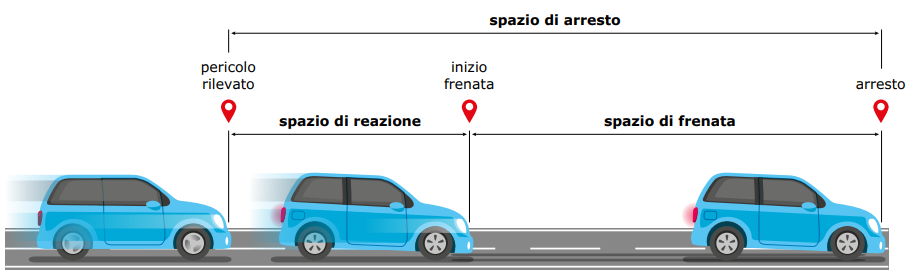
\includegraphics[width=0.9\linewidth]{images/frenata.png}
\centering
\caption{Spazio di arresto}
\end{figure}
